
The identification and reconstruction step relies on the properties that particles display when they interact with the different components of the detector
described in Section~\ref{sec:exp.atlas}.
Once the particle is identified, it is desirable to determine its momentum and
 its origin among other properties.
The important part for the analysis is how well these objects are reconstructed which can be determined by measuring the reconstruction and 
identification efficiencies as a function of kinematic particles, 
usually \pt and $\eta$.
In the next sections we briefly describe how the main physics objects used in 
this analysis are identified and their efficiencies.

\subsection{Basic Principle}

In this section we describe the higher-level reconstruction of particles
as they interact with the different components of the detector.
The schematic of Figure~\ref{fig:exp.atlas.reco.det} 
summarizes the signatures of the different particles in the ATLAS 
detector.



\begin{figure}[htb!]
\centering
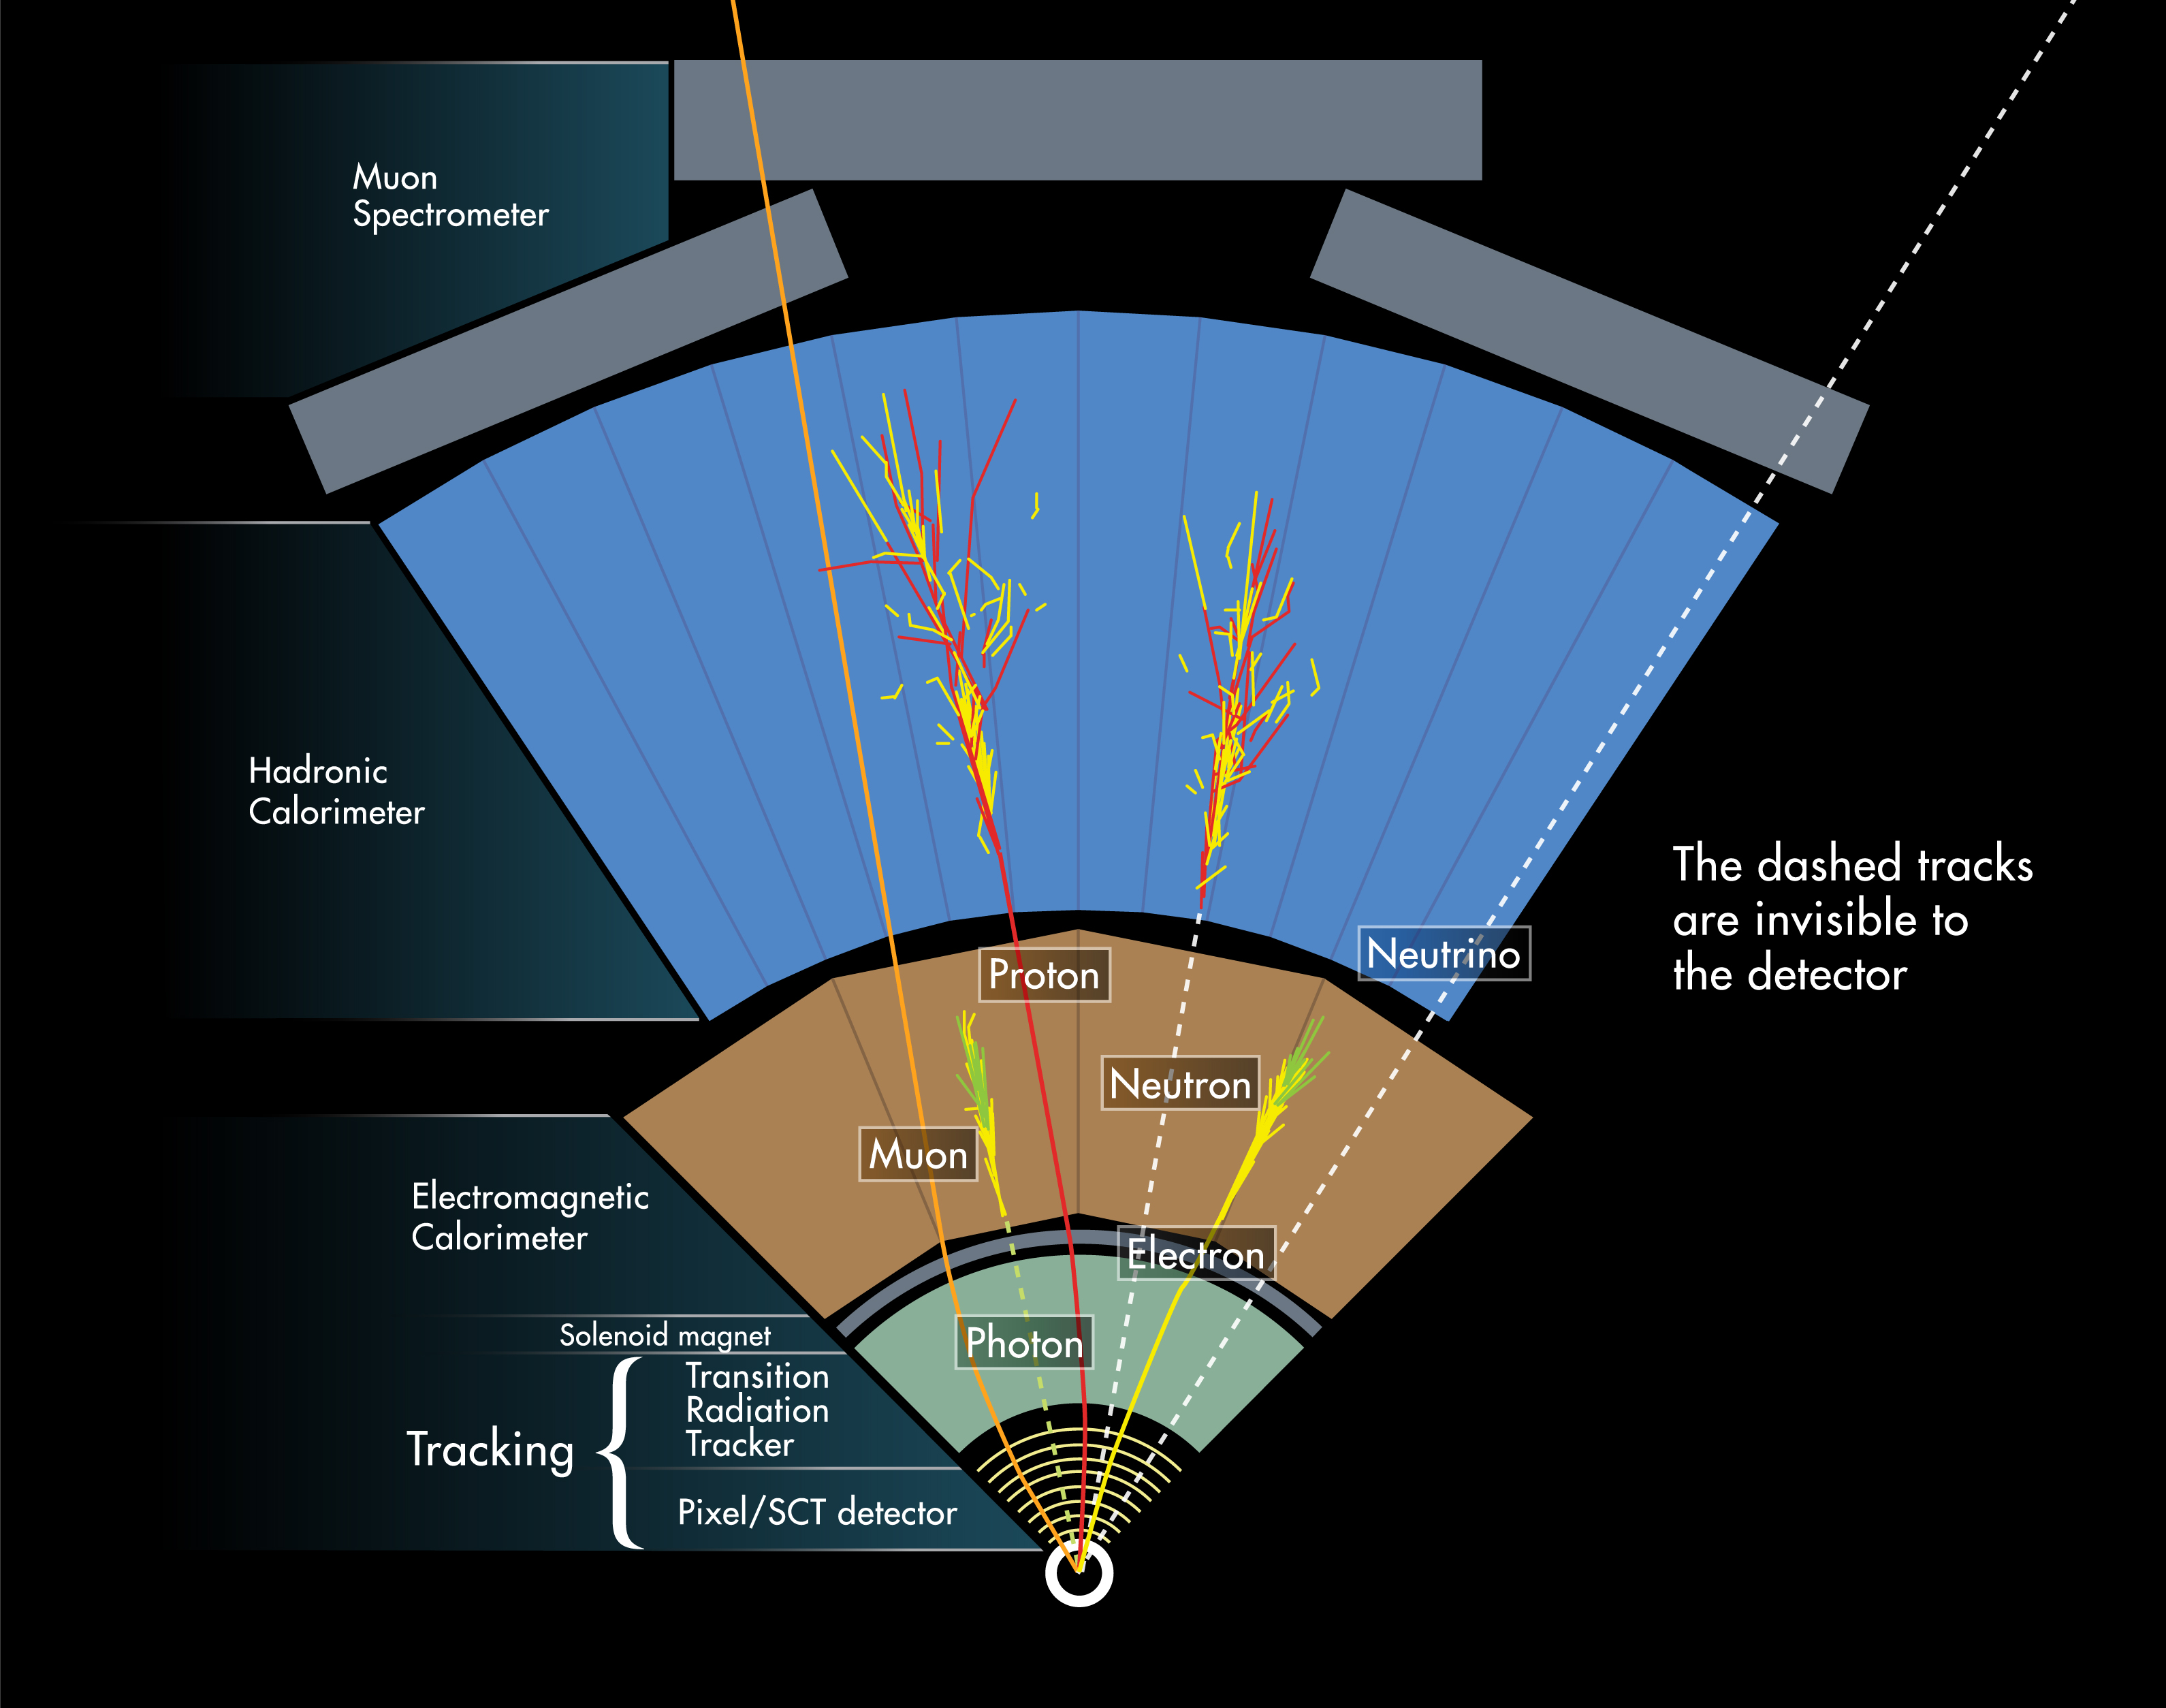
\includegraphics[width=0.95\textwidth]{reco_det.jpg}
\caption{ The different signatures of particles traversing 
the detector are shown in the transverse plane of the ATLAS detector.}% cite??.}
\label{fig:exp.atlas.reco.det}
\end{figure} 


The most important reconstructed particles for the analysis presented 
in this dissertation are charged leptons. 
Charged leptons come from  electroweak processes and  
provide  clear signals which can be accurately reconstructed.
In the remainder of this dissertation, leptons will refer to 
only electrons or muons.

Muons are the simplest to identify since they traverse
the entire ATLAS detector: all other 
interacting particles are stopped before reaching the muon spectrometer.
They are reconstructed as tracks in the inner detector matched to tracks in the
muon spectrometer, 
and leave little energy in the electromagnetic and hadronic calorimeters.  
Muons are produced from decays of $W$ and $Z$ bosons with a relatively 
large momentum, above 15 \GeV, and are produced in isolation from surrounding
detector activity, qualities that we will use in this analysis.
The latter is called ``isolation'' which requires 
the energy of the reconstructed tracks and clusters near the reconstructed 
muon not exceed a certain value. 
This requirement is effective at suppressing muons produced
from background processes such as meson decay in flight and heavy-flavor decay
detailed in Chapter~\ref{chap:fake}.

Electrons are identified by a track in the inner detector that 
initiates  an electromagnetic
shower in the electromagnetic calorimeter. Most of the time,  
all of the energy of the electron is absorbed before reaching the hadronic 
calorimeter.
The electron is identified  by matching reconstructed EM clusters to tracks
reconstructed in the inner detector. 
This signature suffers from 
large backgrounds from other types of charged particles can mimic that 
signature. For these reason, ATLAS uses several tools to effectively 
distinguish between the desired electrons and background.
Similar to muons, isolation is one of these tools.

Photons also produce an electromagnetic shower upon entering the calorimeter, 
except they leave no track in the inner detector since they are neutral.
In practice, photons might undergo a conversion to an $e^+e^-$ pair 
in the detector material before entering the calorimeter which will 
result in a track in the inner detector. Photons of the former case 
are called un-converted, while the latter are called converted photons.
ATLAS has dedicated algorithms to identify photon conversions from 
pairs of reconstructed tracks.% cite??.

Tau leptons are charged particles that decay to the other leptons 
(40\% of the time) or to hadrons (60 \% of the time) before entering the detector.
If they decay to electrons or muons and neutrinos, they are indistinguishable from 
electrons or muons coming from $W$ or $Z$ bosons.
The experimental signatures of hadronically decaying taus are
multiple hadronic showers matched to tracks in the inner detector.
The latter suffers from large backgrounds 
from other types of particles that cannot be suppressed 
as efficiently as background from the leptonic tau decay.


Neutrinos only interact via the weak force
and are thus not directly detected by ATLAS.
As shown in Figure~\ref{fig:exp.atlas.reco.det}, 
they pass through all the sub-detectors.
However, their presence is inferred from an overall 
transverse momentum imbalance of the measured momenta in the event.
Thus, the transverse momentum of the neutrinos can be inferred.
This type of signature is similar to potential new particles 
that will not interact with our detector.
Nevertheless, neutrinos are very well understood
and any potential contribution from them can be accurately 
predicted.

The reconstruction of jets is an essential part of the analysis presented in this dissertation. 
Colored quark and gluons from the primary interaction  undergo a process referred to as hadronization,
where they convert to sprays of colorless hadrons. The collection of this spray of particles is 
referred to as a jet. 
The reconstruction of a jet is based on regrouping of reconstructed clusters and tracks into larger collections using
various clustering algorithms as it will be described next.
By measuring the energy and direction of a jet, we can infer information 
about the initial quarks or gluons that participated in the physics processes under study.
It can also be used to determine the energy of the initial parton in the hard interaction, 
a challenging aspect of jet reconstruction.
The energy of the jet must be calibrated by determining the 
Jet Energy Scale (JES) and the Jet Energy Resolution (JER).% cite??. 
The uncertainties associated with the JES and JER are one of the largest 
experimental uncertainties in this analysis.

The jet reconstruction algorithms cannot determine the type of parton that initiated a
given jet, except for $b$-quarks.
Since $b$-quark hadrons decay with suppressed weak interactions, they are 
relatively long-lived travelling a few millimeters before they decay.
Given the fine tracking resolution of ATLAS, 
a millimeter displacement from the interaction point is large enough to be resolved.
It is thus possible to identify jets containing $b$-hadrons  in a process called ``b-tagging''.
This type of jets, called $b$-jets, are used in this analysis.

More technical details about the reconstruction procedure and the efficiencies 
of the reconstructed objects will be given next.

\subsection{Electrons}
Electrons are reconstructed and identified for $\pt > 5$ \GeV~ and
 $|\eta| < 4.9$ \cite{ATLAS-CONF-2016-024}.
The electrons  are identified by a cluster in the electromagnetic calorimeter 
%of more than 2.5 \GeV~
matched to a track in the inner detector.
The electron trajectory is determined using information from the inner detector. This involves the measurement of the track associated parameters : the
position in the transverse ($d_0$) and longitudinal ($z_0$) planes of the perigee, the particle direction ($\phi$, $\theta$)
and the parameter which provides the inverse track momentum multiplied by the charge ($q/p$). The track
parameters and the associated uncertainties are obtained from the track fitting procedure performed with
the ATLAS Global $\chi^2$ Track Fitter.

The goal is to improve the efficiency of identifying electrons while rejecting background electrons arising from hadronic jets mistaken for electrons, 
electrons from photon conversion, Dalitz decays and from semileptonic heavy-flavour hadron decays.
To do so, three identification (ID) criteria, loose, medium, and tight are defined via likelihoods based on calorimetric cluster shower shapes, 
track and track-to-cluster matching variables.
The tighter the ID criteria, the higher the rejection of background electrons but the lower the identification efficiency.
Figure ~\ref{fig:exp.reco.eff.el} shows the  efficiencies in data and MC for three operating points that are based on a likelihood approach, Loose, Medium and Tight. 
The data efficiencies are obtained by applying data/MC efficiency ratios that were measured in  $J/\psi\to\ee$ and $Z\to\ee$ events to MC simulation. 
The lower efficiency in data than in MC arises from the fact that the MC does not properly represent the 2016 TRT conditions, 
in addition to the known mis-modelling of calorimeter shower shapes in the GEANT4 detector simulation.
The reconstruction efficiency of electrons is around 95\% for low \pt and goes up to 99.9\% for electron $\pt > 45$ \GeV.


\begin{figure}[htb!]
\centering
\begin{subfigure}[t]{0.49\textwidth}
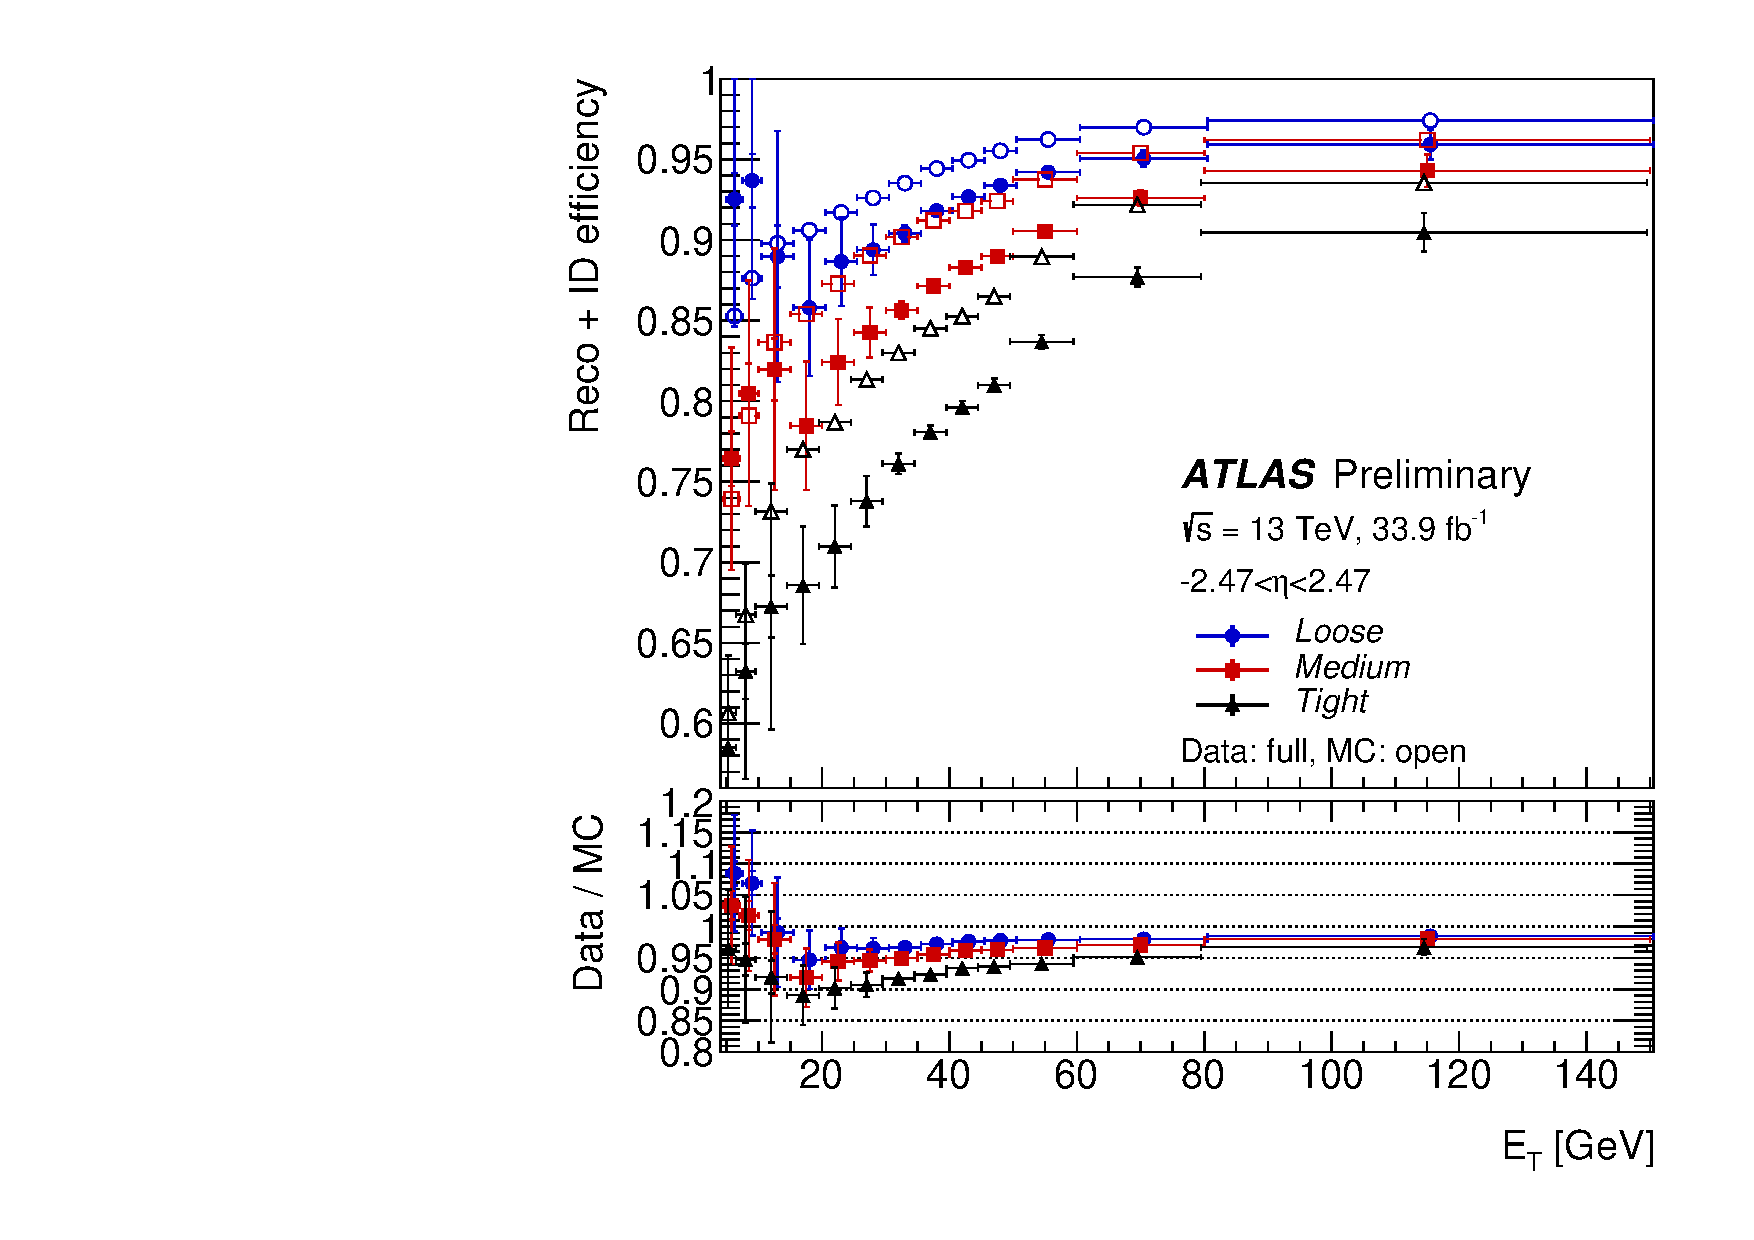
\includegraphics[width=1.\textwidth]{efficiency_pt_el}
\subcaption{}
\label{fig:exp.reco.eff_pt}
\end{subfigure}
\begin{subfigure}[t]{0.49\textwidth}
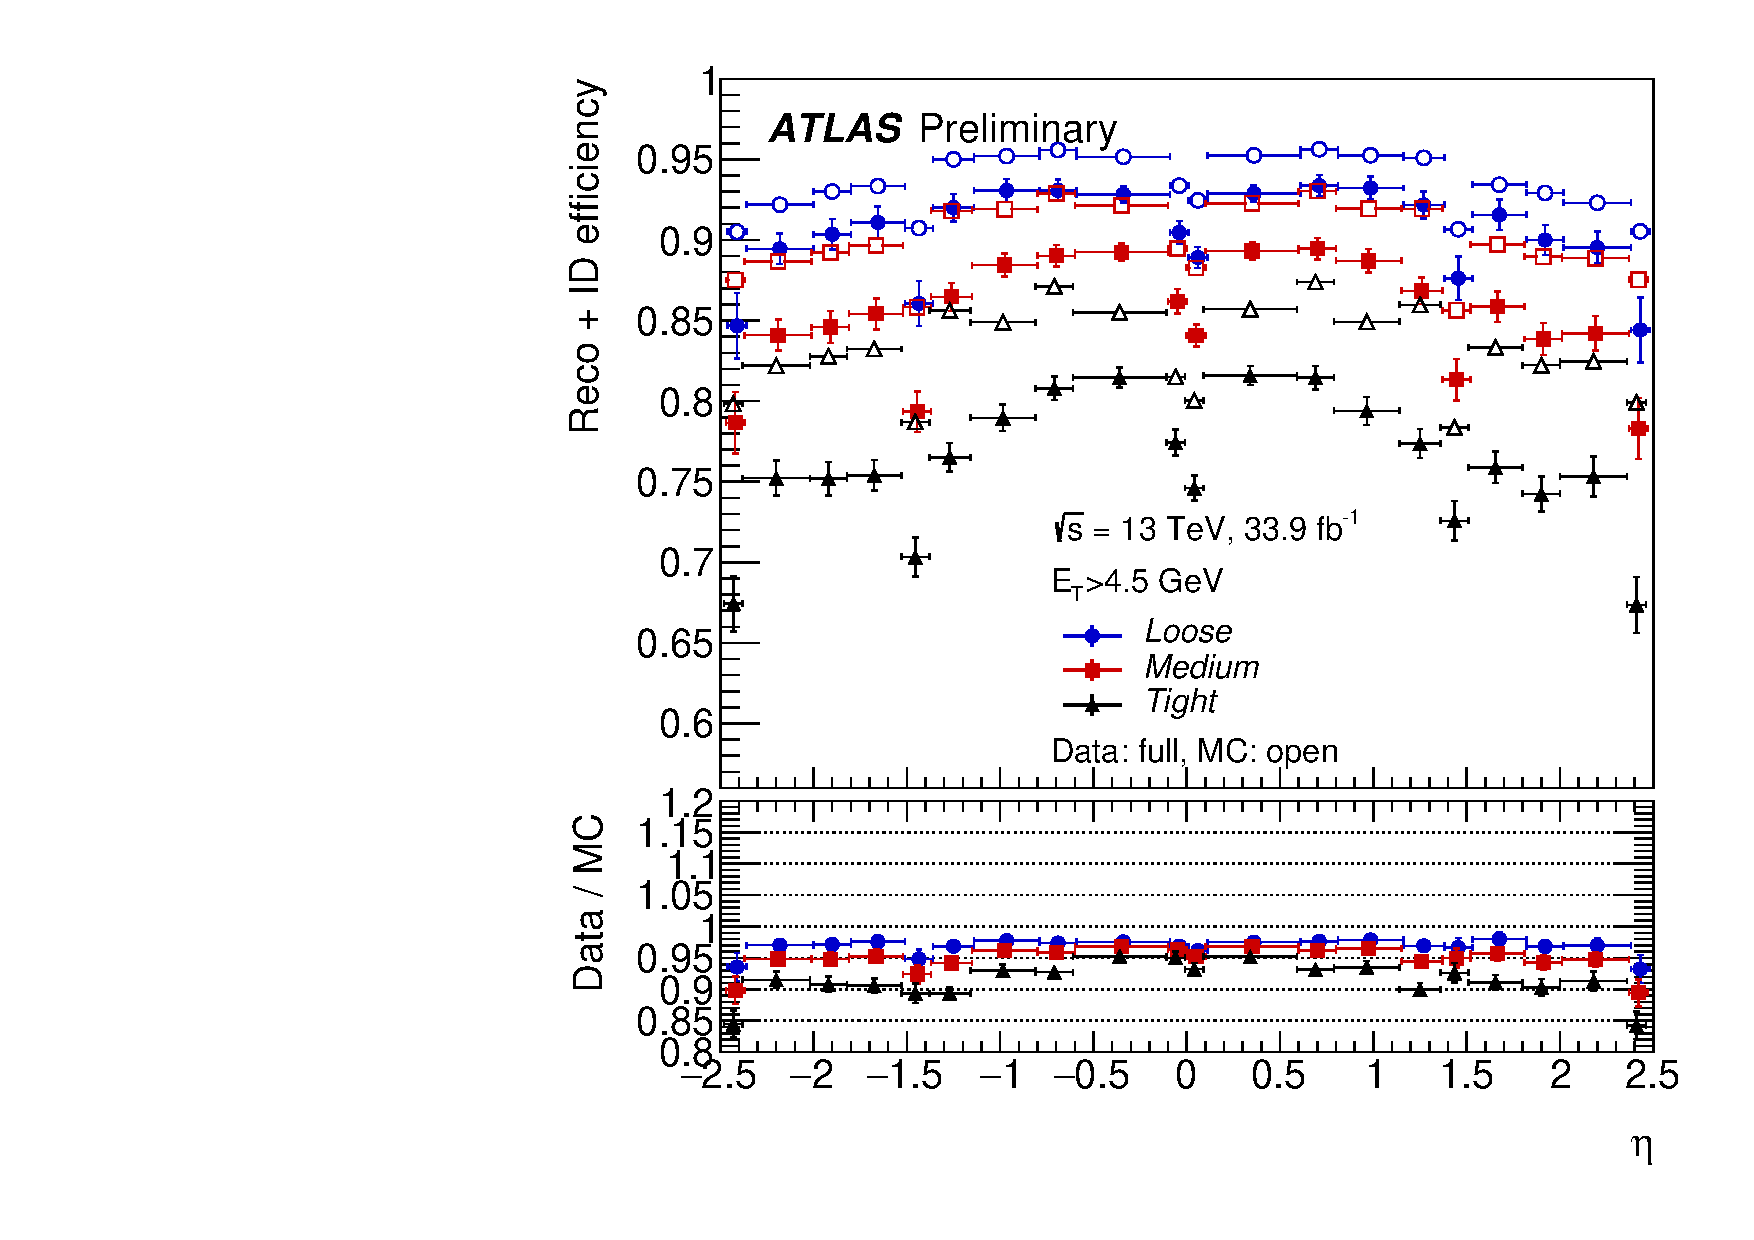
\includegraphics[width=1.\textwidth]{efficiency_eta_el}
\subcaption{}
\label{fig:exp.reco.eff_eta}
\end{subfigure}
%\begin{subfigure}[t]{0.45\textwidth}
%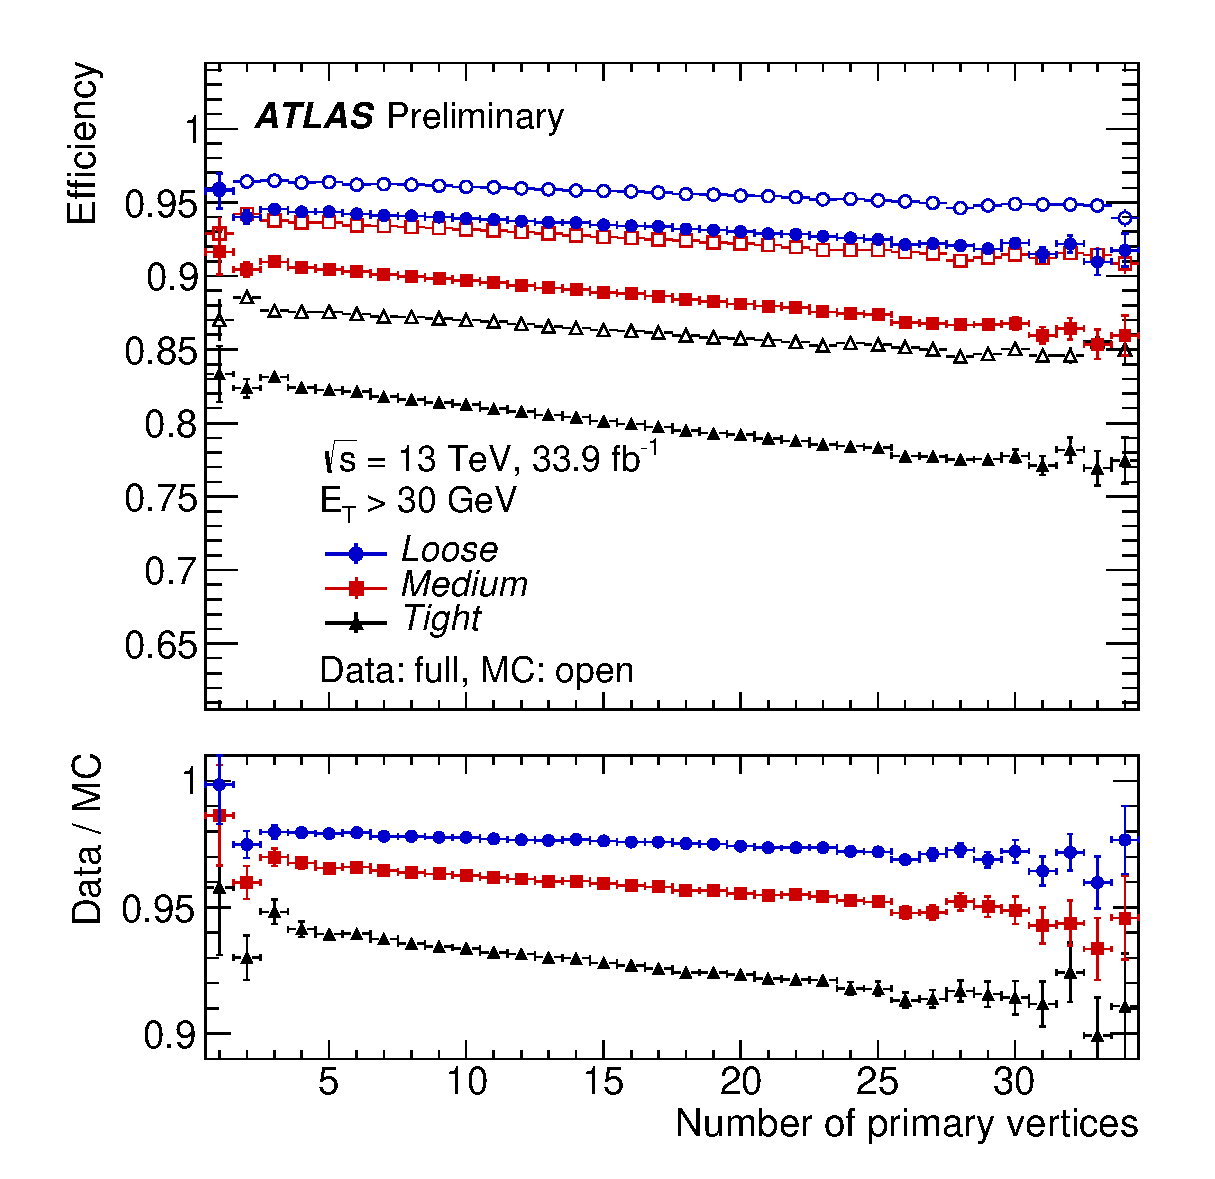
\includegraphics[width=0.95\textwidth]{Nvtx_effSF_el.eps}
%\subcaption{}
%\label{fig:exp.reco.eff_Nvtx}
%\end{subfigure}
\vspace{-0.25cm}
\caption{
Electron reconstruction and identification efficiencies in $Z\to\ee$ events as a function of (a) pseudo-rapidity $\eta$ (b) transverse energy \et.
The total statistical and systematic uncertainty is displayed. 
%(c) number of primary vertices.
}
\label{fig:exp.reco.eff.el}
\end{figure} 

% https://atlas.web.cern.ch/Atlas/GROUPS/PHYSICS/PLOTS/EGAM-2017-003/index.html


To study and compute the corrections needed to account for the detector geometry and material distribution
two sets of MC samples are used. For the first set an ideal geometry (no mis-alignments) with the best
knowledge of the dead material is implemented. For the second scenario, the dead material between the
tracker and calorimeters is increased and the mis-alignments are included. The latter is used to assign the
systematic uncertainties.


%% \begin{figure}[t!]
%% \centering
%% 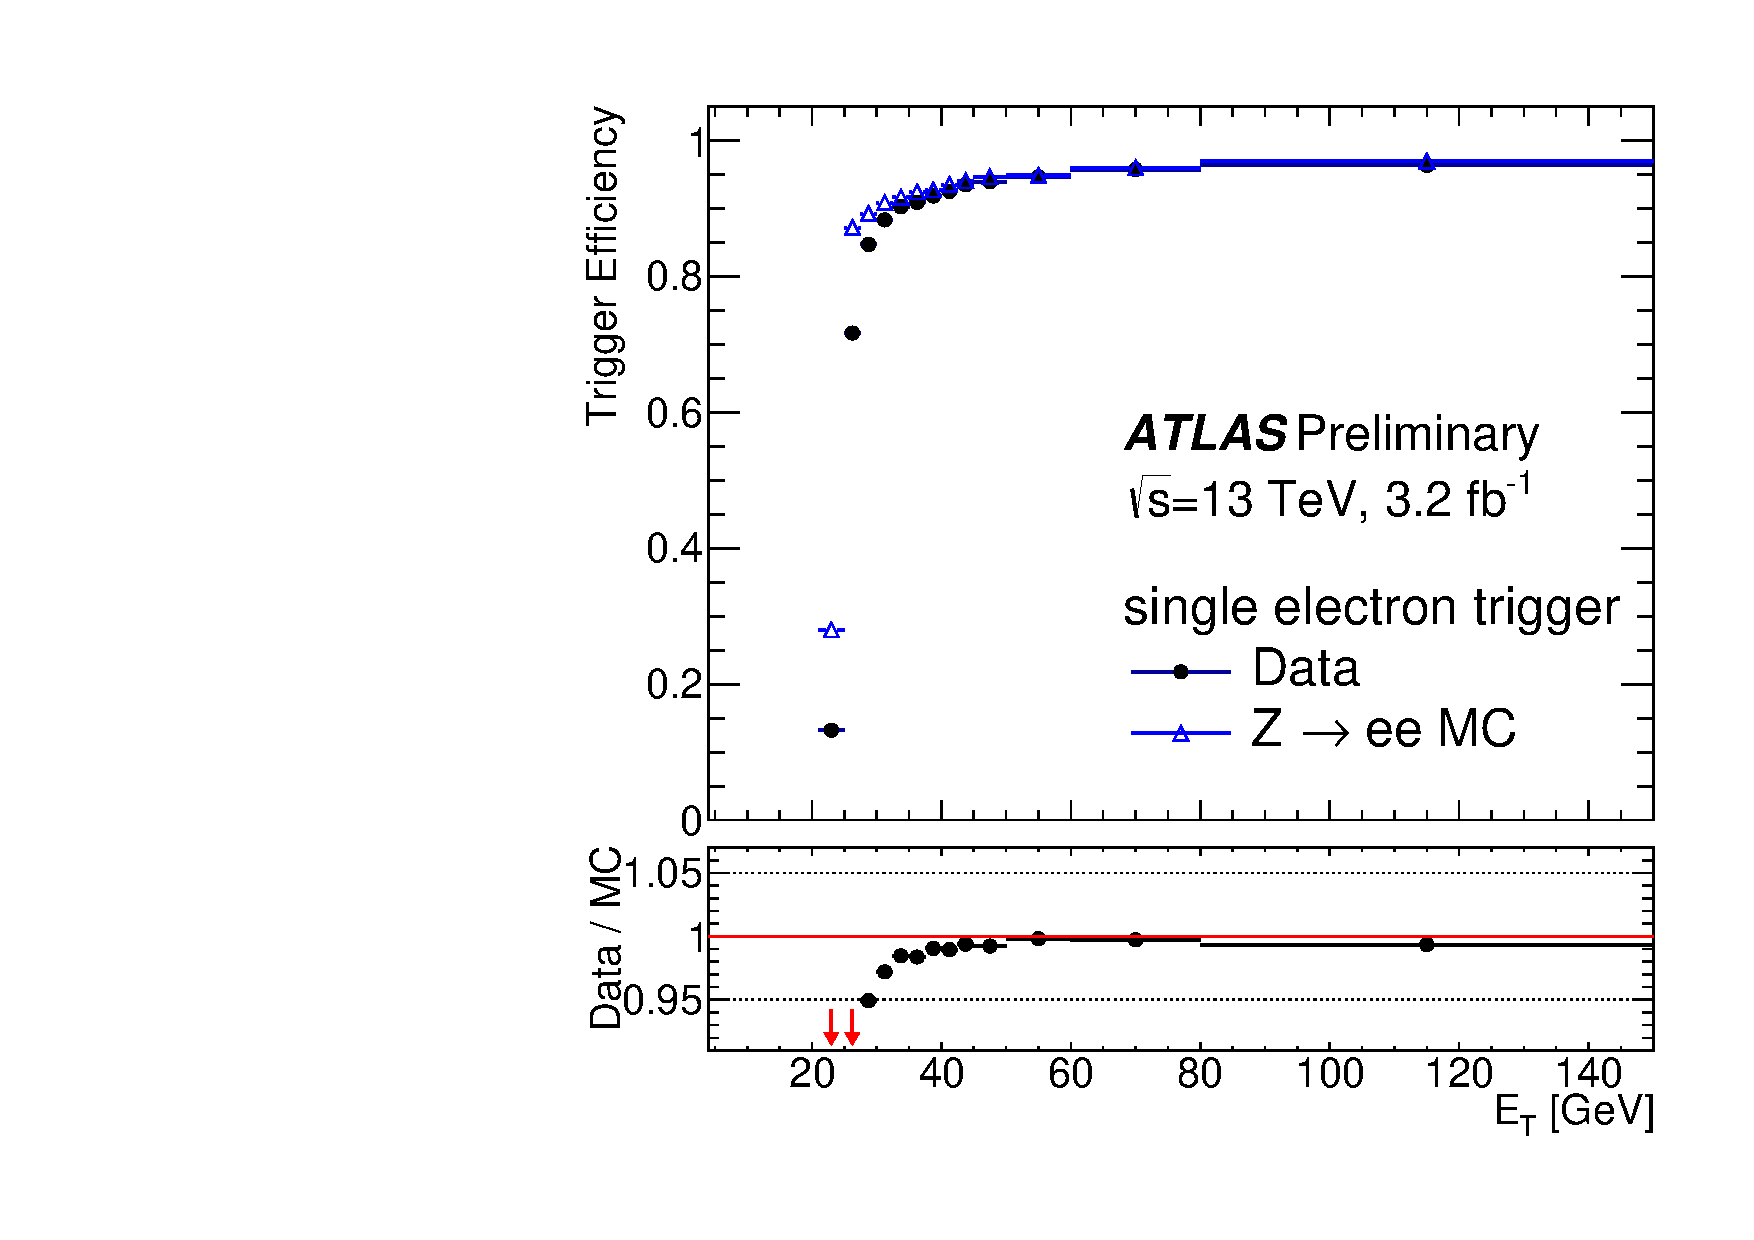
\includegraphics[width=0.95\textwidth]{trigger_eff_el_Et}
%% \caption{}
%% \label{fig:}
%% \end{figure} 



%% \begin{figure}[t!]
%% \centering
%% 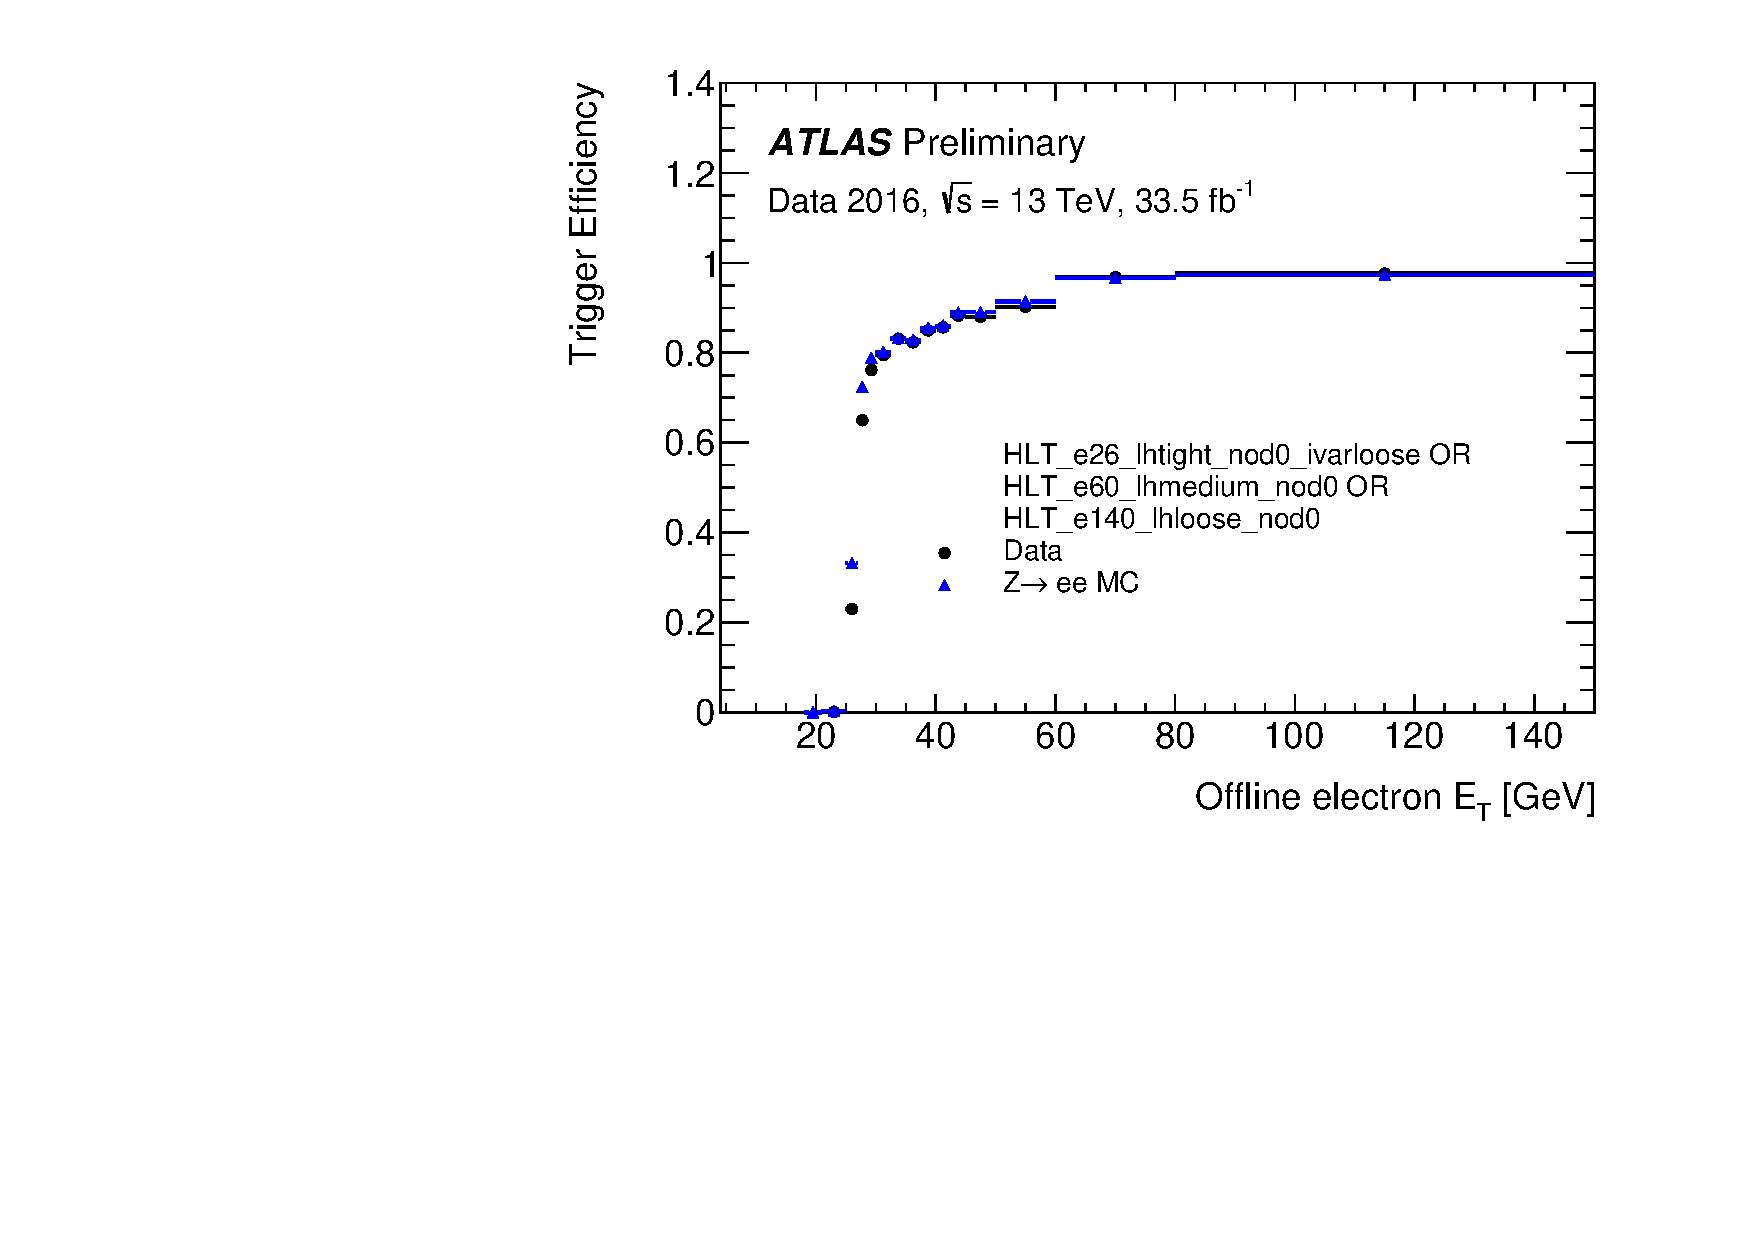
\includegraphics[width=0.95\textwidth]{Eff_Et_singleOR_full2016}
%% \caption{Efficiency of the logical OR between HLT\_e26\_lhtight\_nod0\_ivarloose, HLT\_e60\_lhmedium\_nod0 and HLT\_e140\_lhloose\_nod0 triggers as a function of the offline electron candidate's transverse energy (ET).}
%% \label{fig:}
%% \end{figure} 



\subsection{Muons}

The ATLAS detector has been designed to provide clean and efficient 
muon identification and precise muon momentum measurements over 
a wide range of energy and solid angle. 
The muon  reconstruction starts in the inner 
detector where tracks are identified up to $|\eta|<2.5$ in a solenoidal field of 2 Tesla.
The muon spectrometer  measures  muons up to $|\eta|<2.7$  
providing momentum measurements with a design relative resolution of better than 3\% over a wide 
\pt range and to 10\% at 1 \TeV.
Similar to electrons, four muon identification selections are defined in order to meet 
the specific needs of different physics analyses:
\begin{itemize}
\item loose muons: maximize efficiency: ideal for multilepton final states analysis
\item medium muons: minimize systematics uncertainties
\item tight muons: optimize  purity
\item high-\pt muons: maximize momentum resolution for high \pt tracks ($>100$ \GeV)  
\end{itemize}
Figure~\ref{fig:exp.reco.muon} shows the reconstruction efficiency of the muon for different selections measured in  $Z\to\mu\mu$ and $J/\psi\to\mu\mu$ events.

The reconstruction efficiency is measured to be close to 99\% over most of the phase space relevant for the analysis. 
The isolation efficiency is between 93\% and 100\% based on the selection and muon momentum. The simulation reproduce both efficiencies very well.
The  momentum resolution is measured to be as low as 1.7\% and the momentum scale uncertainty is less than  0.05\%.

\begin{figure}[htb!]
\centering
\begin{subfigure}[t]{0.56\textwidth}
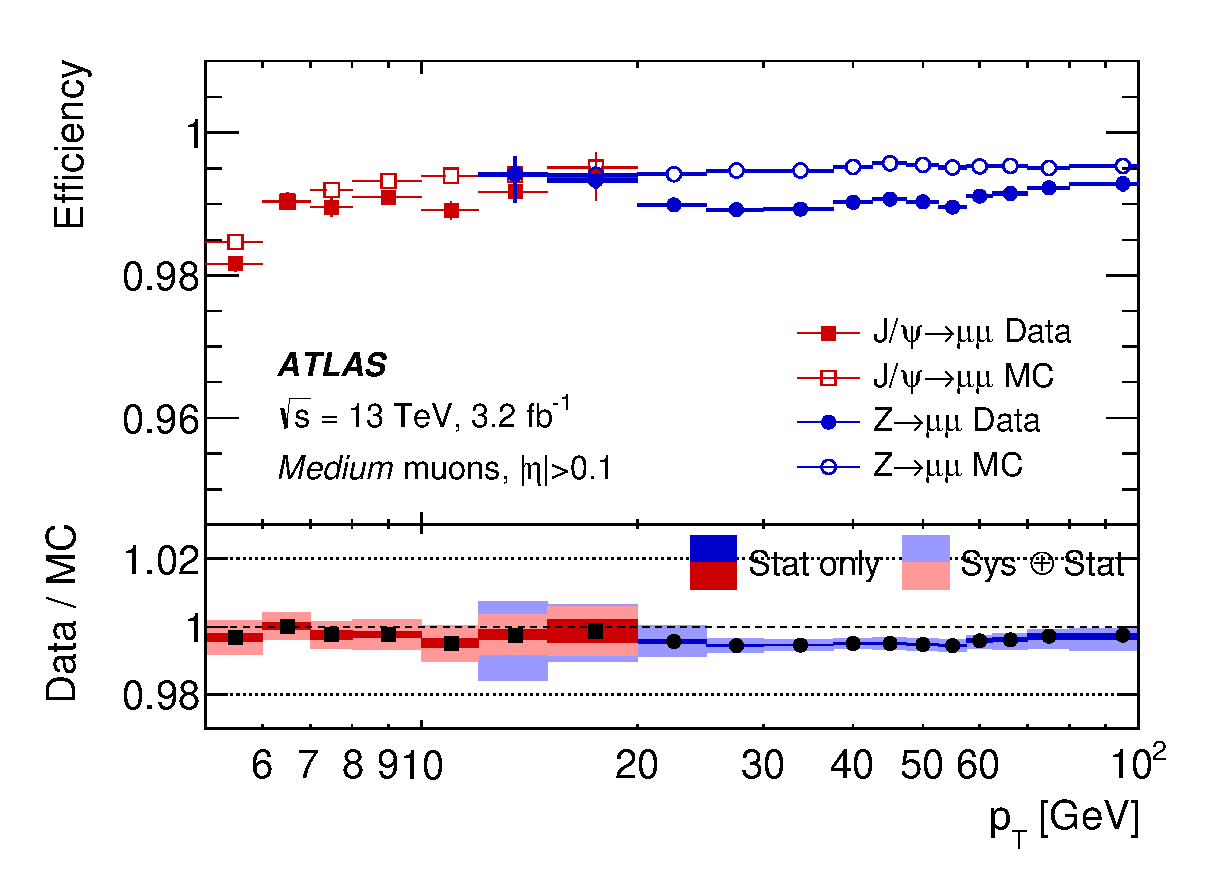
\includegraphics[width=1.\textwidth]{EffwMedium_pt_muons.eps}
\subcaption{}
\label{fig:}
\end{subfigure}
\begin{subfigure}[t]{0.43\textwidth}
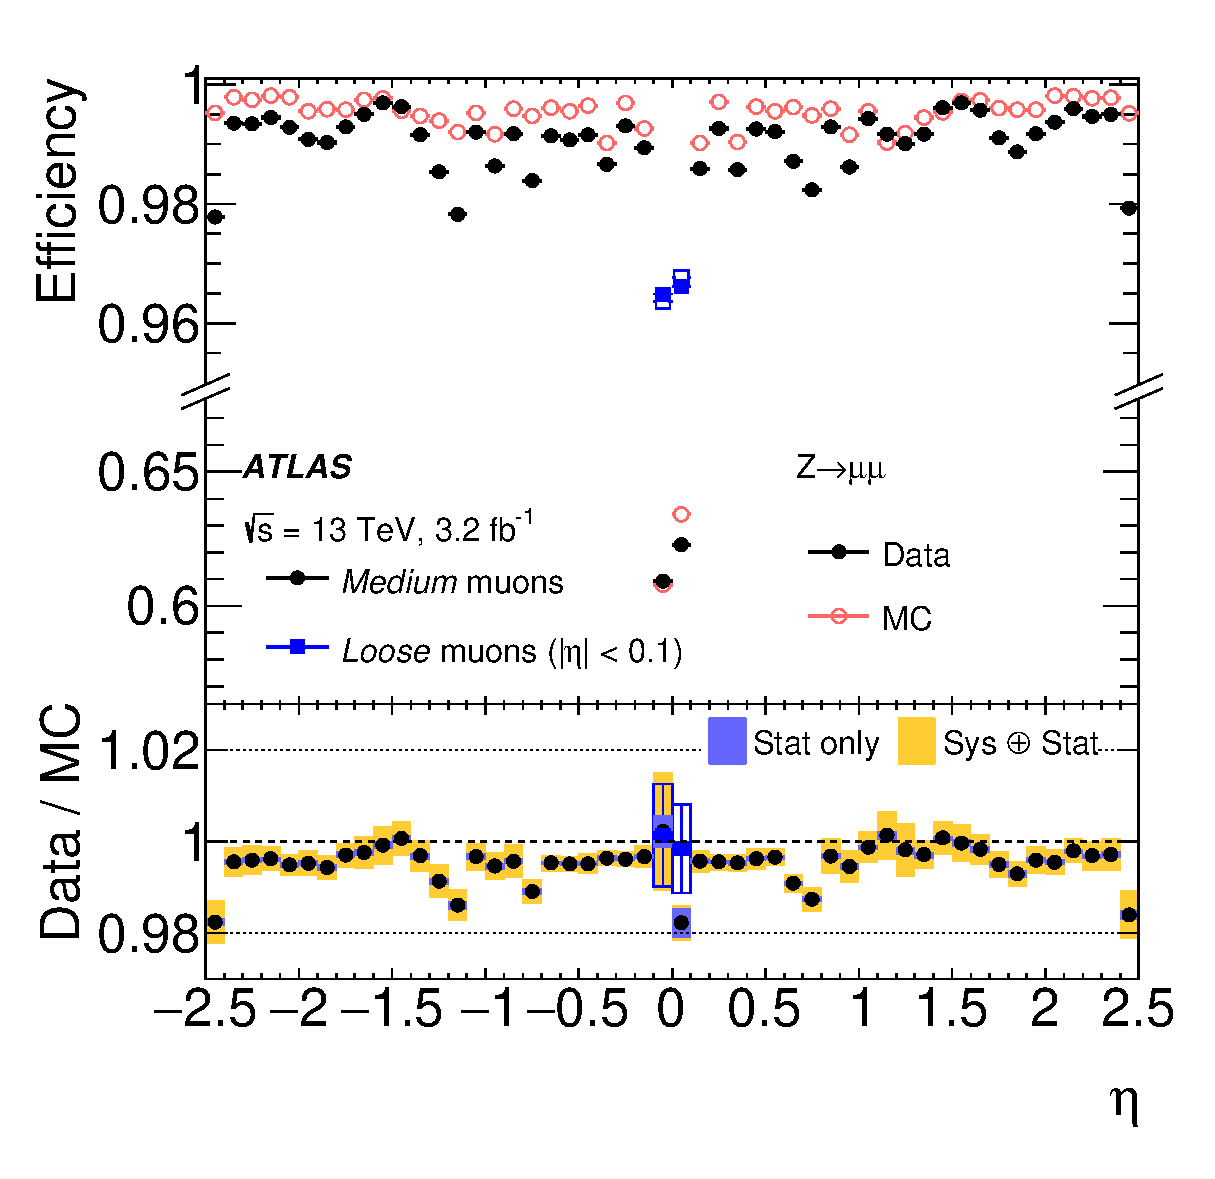
\includegraphics[width=1.\textwidth]{EffwLoose_Medium_Eta_muons.eps}
\subcaption{}
\label{fig:}
\end{subfigure}
\vspace{-0.25cm}
\caption{(a) Reconstruction efficiency for the medium muon selection as a function of (a) \pt (b) $\eta$ of the muon.
 The error bars on the efficiencies indicate the statistical uncertainty. The panel at the bottom shows the ratio of the measured to predicted efficiencies, with statistical and systematic uncertainties.
%(b) Muon reconstruction efficiency as a function of $\eta$ measured in $Z\to\mu\mu$ events for muons with $\pt>10$ \GeV~shown for the Medium muon selection. In addition, the plot also shows the efficiency of the Loose selection (squares) in the region $|\eta|<0.1$ where the Loose and Medium selections differ significantly. The error bars on the efficiencies indicate the statistical uncertainty. Panels at the bottom show the ratio of the measured to predicted efficiencies, with statistical and systematic uncertainties. 
}
\label{fig:exp.reco.muon}
\end{figure} 


\subsection{Jets}
Jets are reconstructed using the anti-$k_{t}$ jet algorithm~\cite{Cacciari:2008gp} 
with the distance parameter $R$ set to $0.4$ and 
a three dimensional input of topological energy clusters in the 
calorimeter~\cite{PERF-2014-07}. 
The advantage of using the anti-$k_{t}$ algorithm is that it is infrared
 and collinear safe\footnote{These two problems arise when defining a seed used 
as a starting point of an iterative process of re-clustering energy 
depositions in the calorimeter cells.
If only particles above some momentum threshold are used as seeds then the 
procedure is collinear unsafe. On the other hand, if the addition of an 
infinitely soft particle leads to a new stable energy cone being found then 
the procedure is infrared unsafe.
}.
It is also resilient to soft-QCD emissions, a process that is common in the hadron colliders.
The jets are constructed by defining two distances:
\begin{itemize}
\item $d_{ij} = \min\left((k_{kj}^{2p},k_{kj}^{2p}\right)\frac{\Delta_{ij}^2}{R^2}$: the distance between two particles i and j.
\item $d_{iB} = k_{ti}^{2p}$: the distance between a particle $i$ and the beam $B$.
\end{itemize}
where $\Delta_{ij}^2 = \left( y_i - y_j\right)^2 + \left(\phi_i - \phi_j\right)^2$ and $k_{ti}$, $y_i$, and $\phi_i$ are the transverse momentum, rapidity, and azimuth of the 
particle $i$. The radius parameter $R$ scales $d_{ij}$ with respect to $d_{iB}$ such that any pair of final jets $a$ and $b$ are separated by at least $R^2=\Delta_{ab}^2$.
The parameter $p$ governs the relative power of of energy with respect to the geometrical scales, and is set to $p=-1$ for the anti-$k_{t}$ algorithm.


The energies of the jets are calibrated to  account the necessary losses associated with sampling calorimeter,
the presence of dead material,  energy loss in non-instrumented regions, etc. This is performed using the local cluster weighting
(LCW) scheme \cite{Aad:2016upyew}, which uses calibrated topological clusters as input to the anti-$k_{t}$ jet algorithm,
and takes into account jet energy scale (JES) and jet energy resolution (JER) calibrations.
Both JES and JER can have an important contribution to the systematic uncertainties of this analysis.
The fractional JES uncertainty in Figure~\ref{fig:exp.JES_pt_sys} shows that jets with \pt below 50 \GeV~can have a larger uncertainty.
The choice was made to only require jets above 50 \GeV~in the analysis for this reason.
The fractional JER is around 17\% for jets with \pt of 30 \GeV~decreasing down to 5\% for more energetic jets.
An additional variable is used to suppress jets from pileup, called the jet vertex tagger (JVT).
JVT is a multivariate combination of the fraction of the total momentum of tracks in the jet which is associated with the primary vertex
and  track-based variables to suppress pileup jets \cite{ATL-PHYS-PUB-2015-034}. 

\begin{figure}[htb!]
\centering
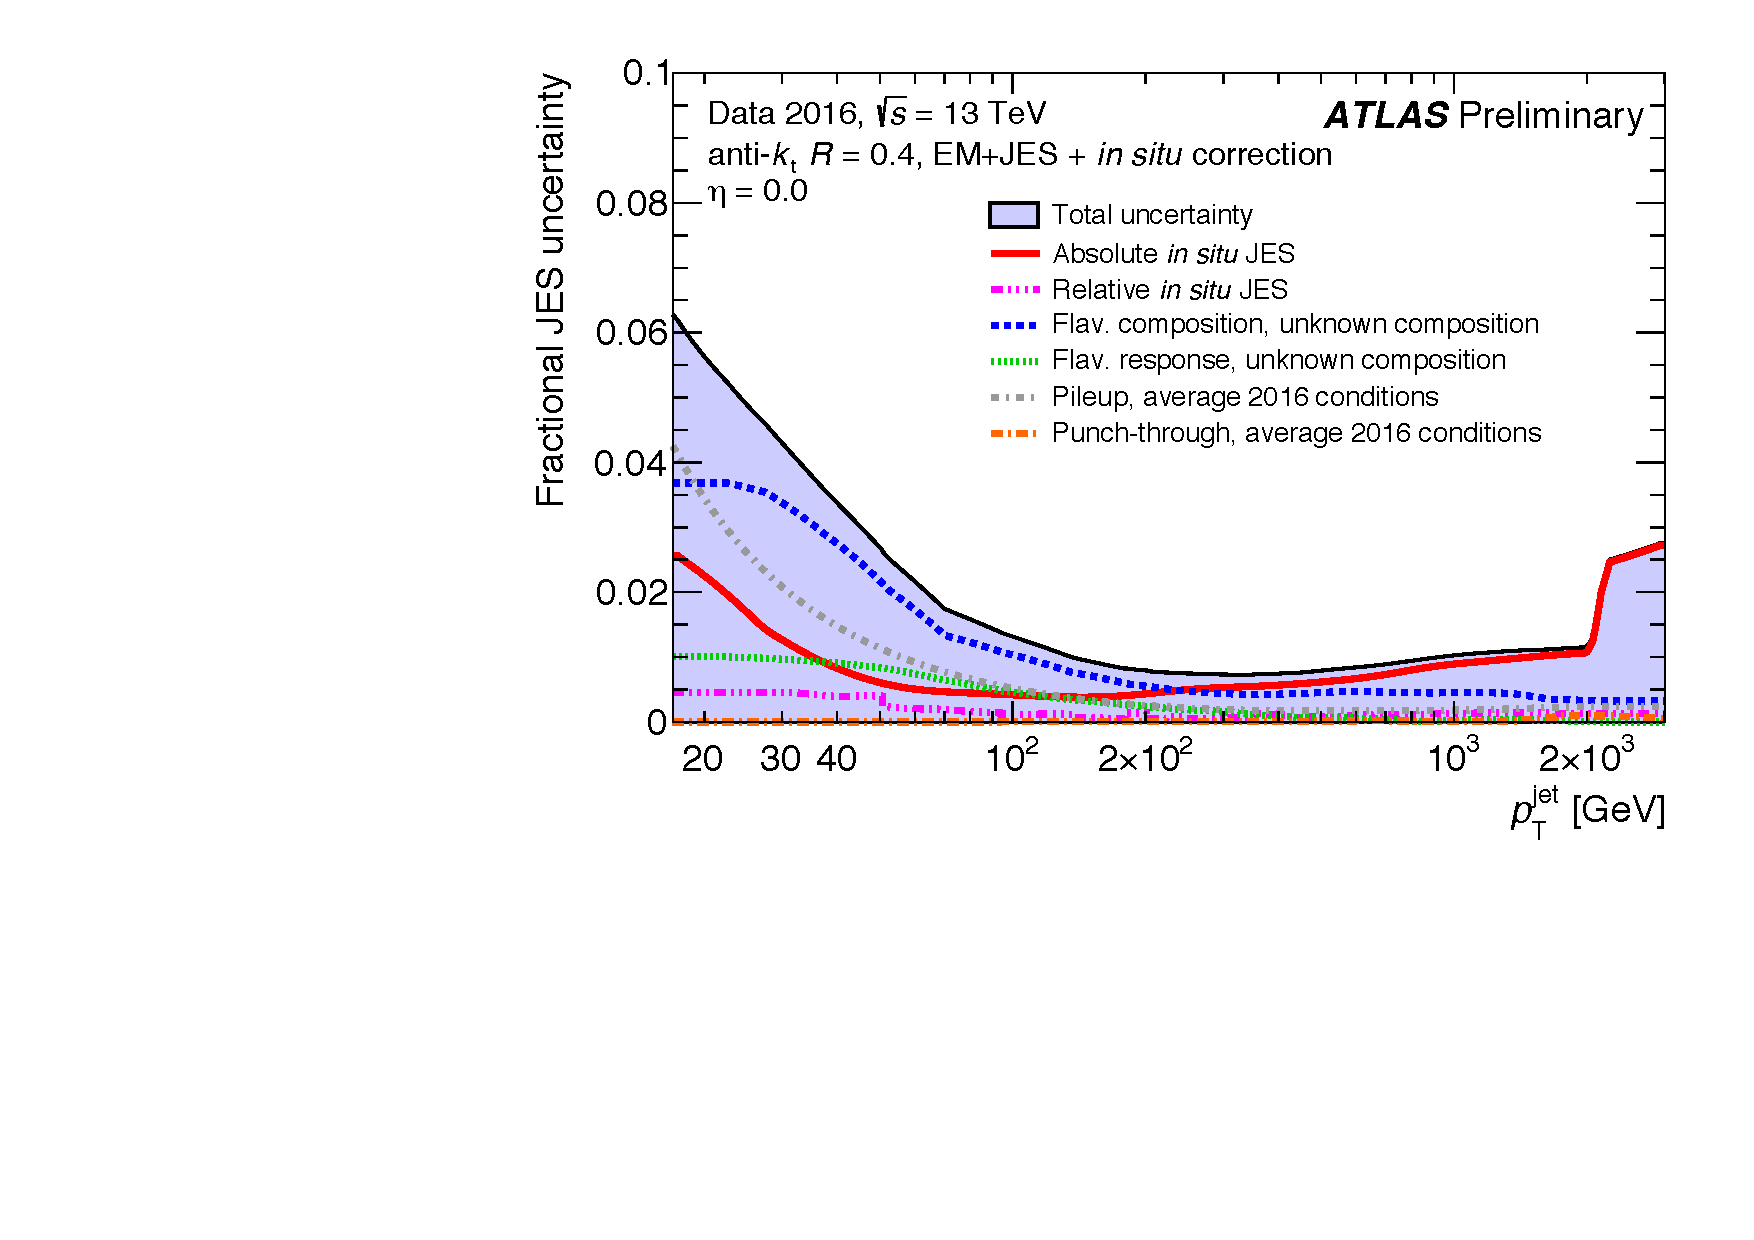
\includegraphics[width=0.65\textwidth]{JES_pt_sys}
\caption{Fractional jet energy scale systematic uncertainty components as a function of \pt for anti-$k_{t}$ jets at $\eta$ = 0.0 
with distance parameter of $R$ = 0.4 after calibration.
The total uncertainty (all components summed in quadrature) is shown as a filled blue region topped by a solid black line.}
\label{fig:exp.JES_pt_sys}
\end{figure} 

%% The reconstruction efficiency 

%% \begin{figure}[t!]
%% \centering
%% \begin{subfigure}[t]{0.48\textwidth}
%% 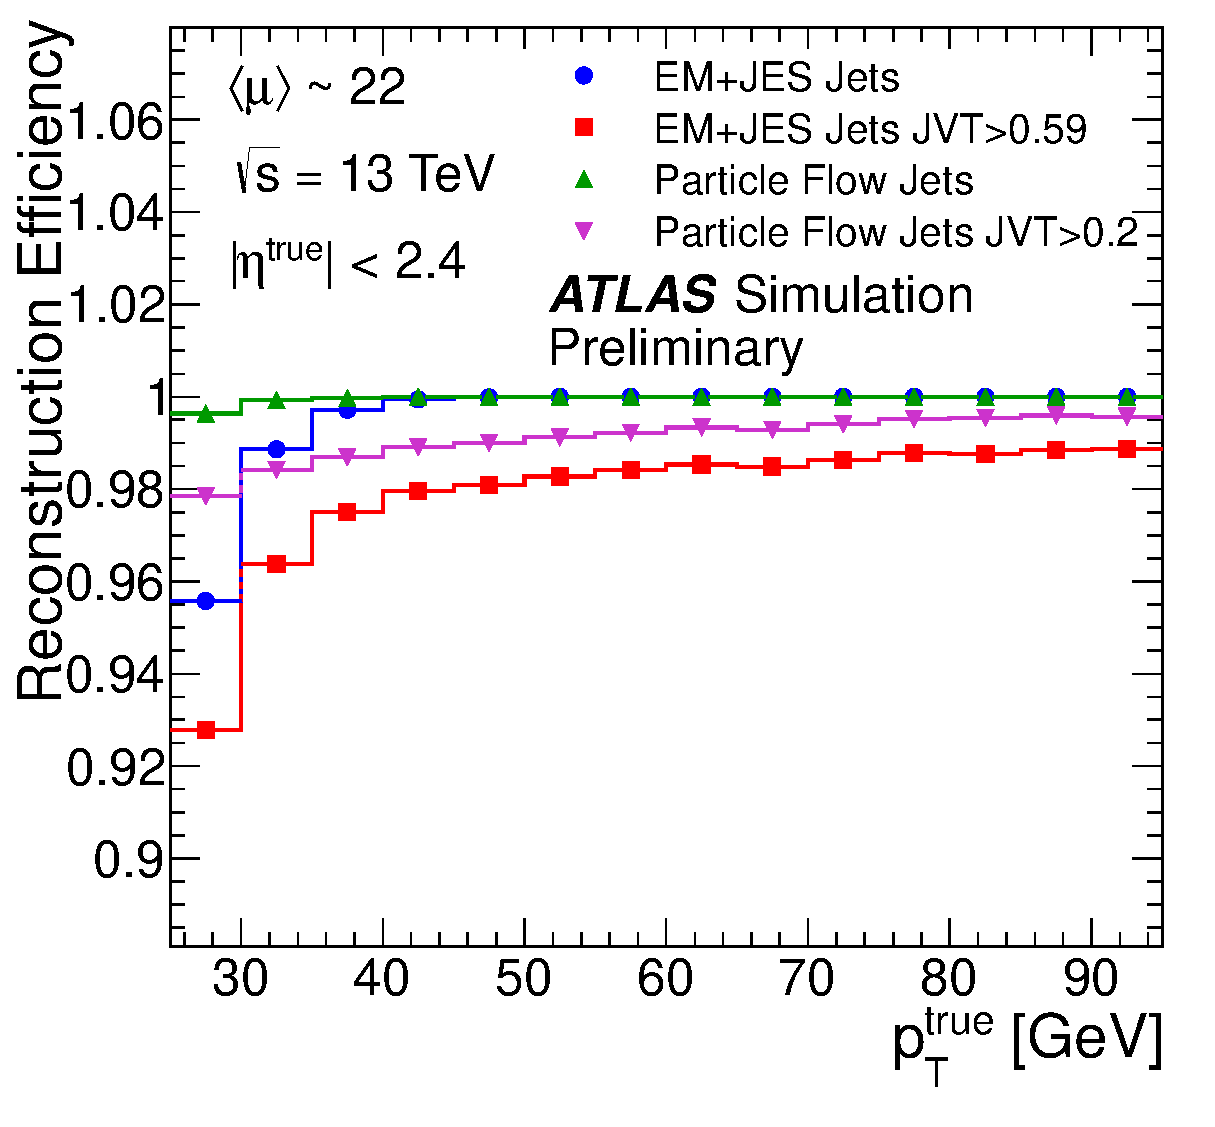
\includegraphics[width=0.95\textwidth]{Eff_pt_jets.eps}
%% \subcaption{}
%% \label{fig:}
%% \end{subfigure}
%% \begin{subfigure}[t]{0.48\textwidth}
%% 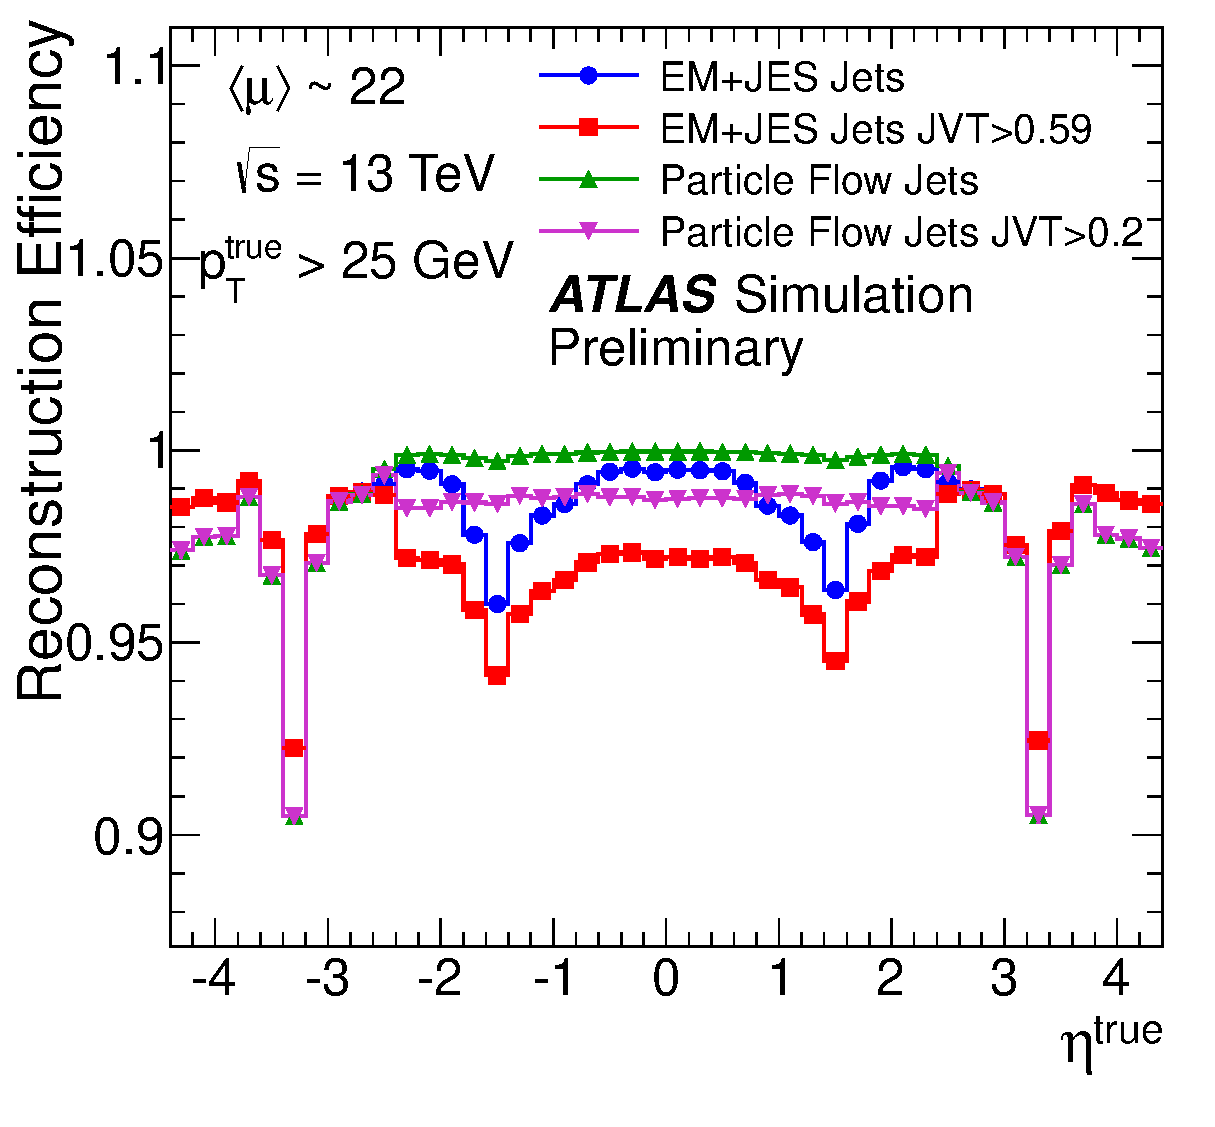
\includegraphics[width=0.95\textwidth]{Eff_eta_jets.eps}
%% \subcaption{}
%% \label{fig:}
%% \end{subfigure}
%% \vspace{-0.25cm}
%% \caption{
%% The efficiency of reconstructing a hard-scatter truth particle jet (reconstructed jet found within $\Delta R<0.4$ with $\pt^\text{jet}>10 $\GeV) within $|\eta^\text{true}|<2.4$ as a function 
%% of $\pt^\text{true}$. Two reconstruction methods are shown; EM+JES calorimeter jets [arXiv:1703.09665], and Particle Flow jets [arXiv:1703.10485]. Also shown are both jet collections with a 
%% Jet Vertex Tagger (JVT) [arXiv:1510.03823] requirement applied to reduce the fake jet rate. While the plot shows the effect of the cuts for the full spectrum, typically JVT requirements are 
%% only applied for $\pt^\text{jet}<60$ \GeV. 
%% Jets are only reconstruted if after the jet area pile-up correction their \pt is above 5 GeV. Simulated samples are Powheg+Pythia8 $Z\to\mu\mu$ events with pile-up overlaid with conditions 
%% similar to the data-taking in 2016, with a mean average number of interactions per crossing of 22.
%% }
%% \label{fig:}
%% \end{figure} 




\subsection{Heavy flavor}

The jet reconstruction algorithms cannot identify which type of parton initiated the jet except in the case of 
jets containing $b$-hadrons. 
Bottom-quark flavored hadrons live relatively longer which gives them specific characteristics that can be used 
to identify them. The procedure is commonly referred to as $b$-tagging and
is performed with the MV2 algorithm, a multivariate discriminant making 
use of track impact parameters 
and reconstructed secondary vertices~\cite{Aad:2015ydr,ATL-PHYS-PUB-2015-022}
to provide the best separation among the different jet flavour hypotheses.
An example of the output of the multivariate discriminant is shown in Figure~\ref{fig:exp.btag.bdt} 
where typically a cut must be applied on the score to identify an operating working point. 
%The notation MV2cxx denotes the faction $xx$ of c-jet contribution present in the training.
Three MV2 algorithms were released that correspond to MV2c00, MV2c10, and 
MV2c20.
MV2c00 denotes the MV2 algorithm where no c-jet contribution was present in the training and MV2c10 (MV2c20) denote the MV2 outputs where a 7\% (15\%) c-jet fractions was present 
in the background sample.
The performance of the optimized  MV2c00, MV2c10 and MV2c20 b-tagging algorithms is shown in Figure~\ref{fig:exp.btag.eff}
for the c-jet rejection as a function of the b-jet efficiency.
The MV2c20 is the best performing algorithm leading to an optimal rejection of c-jets at a given b-tagging 
efficiency. As a result, it is the algorithm used in this analysis.


\begin{figure}[htb!]
\centering
\begin{subfigure}[t]{0.48\textwidth}
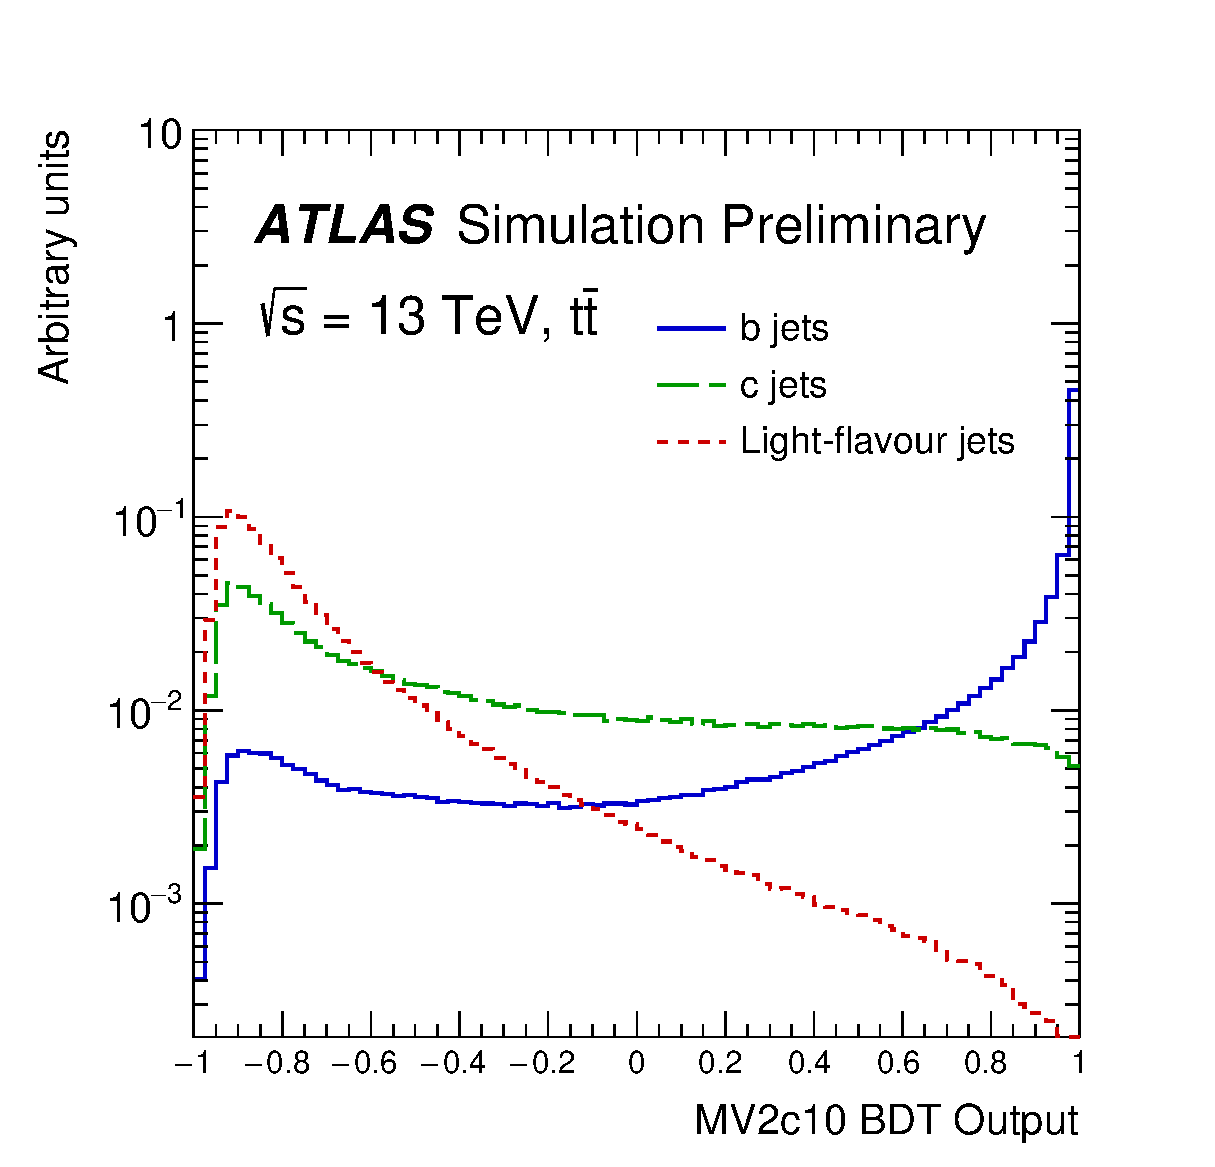
\includegraphics[width=0.95\textwidth]{btag_bdt}
\subcaption{}
\label{fig:exp.btag.bdt}
\end{subfigure}
\begin{subfigure}[t]{0.48\textwidth}
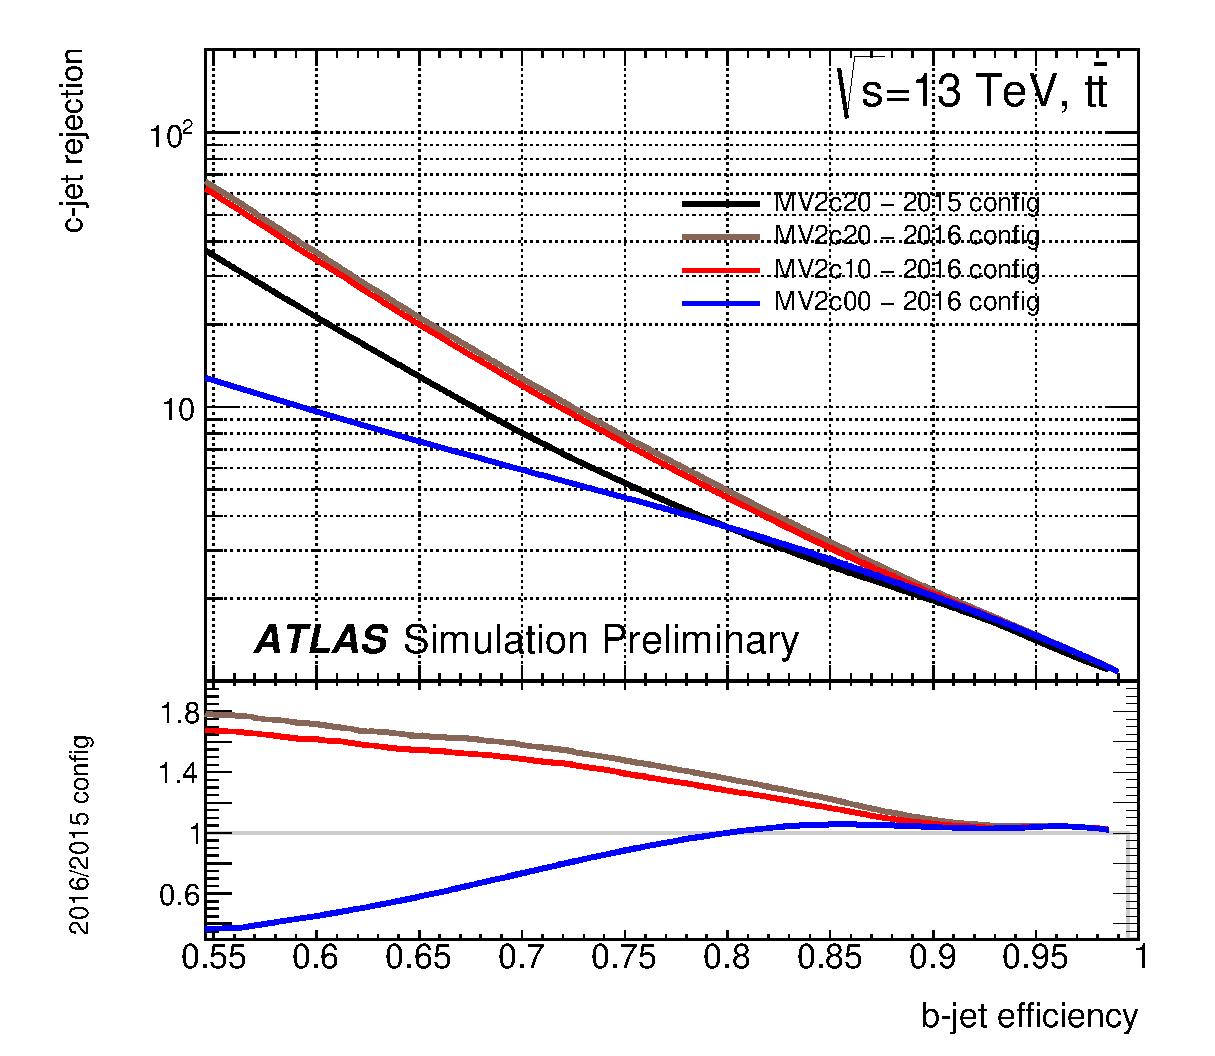
\includegraphics[width=0.95\textwidth]{btag}
\subcaption{}
\label{fig:exp.btag.eff}
\end{subfigure}
\vspace{-0.25cm}
\caption{
(a) MV2c10 BDT output for b- (solid blue), c- (dashed green) and light-flavour (dotted red) jets evaluated with tt events. 
(b) c-jet rejection versus b-jet efficiency for the 2015 and 2016 configurations of the algorithm.
 (for the 2016 configuration). 
}
\label{fig:exp.btag}
\end{figure} 


\subsection{Missing transverse momentum}
The missing transverse momentum is an important quantity in searching for new physics scenarios which expect a stable, 
non-electromagnetically, and non-hadronically interacting 
particle. Such a particle does not interact with the detector and can only be identified through an imbalance of the momentum 
distribution between the particles 
of the event. 
Since the momentum of the colliding protons is almost completely along the beam, longitudinally, 
the transverse component of the momenta of the 
scattered objects should add up to zero.
Based on the conservation of momentum, the sum of all visible four momenta projected in the transverse plane should be close to zero if 
no particles are missed.
However, this quantity will be large if a particle, potentially from new physics models, escaped detection. 
The missing transverse momentum is defined as the negative vector sum of the transverse momenta of the visible reconstructed objects in the
 event: 
\begin{equation}
\pt^{\rm{miss}} = - \sum_\text{visible} \pt
\end{equation}
where the visible objects include electrons, muons, jets, photons, taus, and a soft term.
In the rest of the dissertation, the magnitude of the missing transverse momentum vector is denoted by \met.
The soft term  is  a fundamental quantity in the reconstruction of \met and be estimated by 
\begin{itemize}
\item Calorimeter based Soft Term (CST): accounts for both neutral and charged particle energies.
\item Track based Soft Term (TST): incorporates a natural pileup suppression by selecting only tracks from primary vertices.
\end{itemize}

The \met performance depends on the event topology affected by the presence of true \met, from neutrinos for example,
charged leptons, jet activity, and others.
The \met performance is generally studied with processes with and without genuine \met, such as 
$W \to e \nu$ and $Z\to\mu\mu$ events. 
The scale and resolution for the reconstructed \met in these processes are indicative of the reconstruction quality.
For illustration, results obtained with  $Z\to\mu\mu$ events are shown in Figure~\ref{fig:exp.reco.met}.
Generally, the \met has a resolution in the order of 10 to 20 \GeV.


\begin{figure}[htb!]
\centering
\begin{subfigure}[t]{0.48\textwidth}
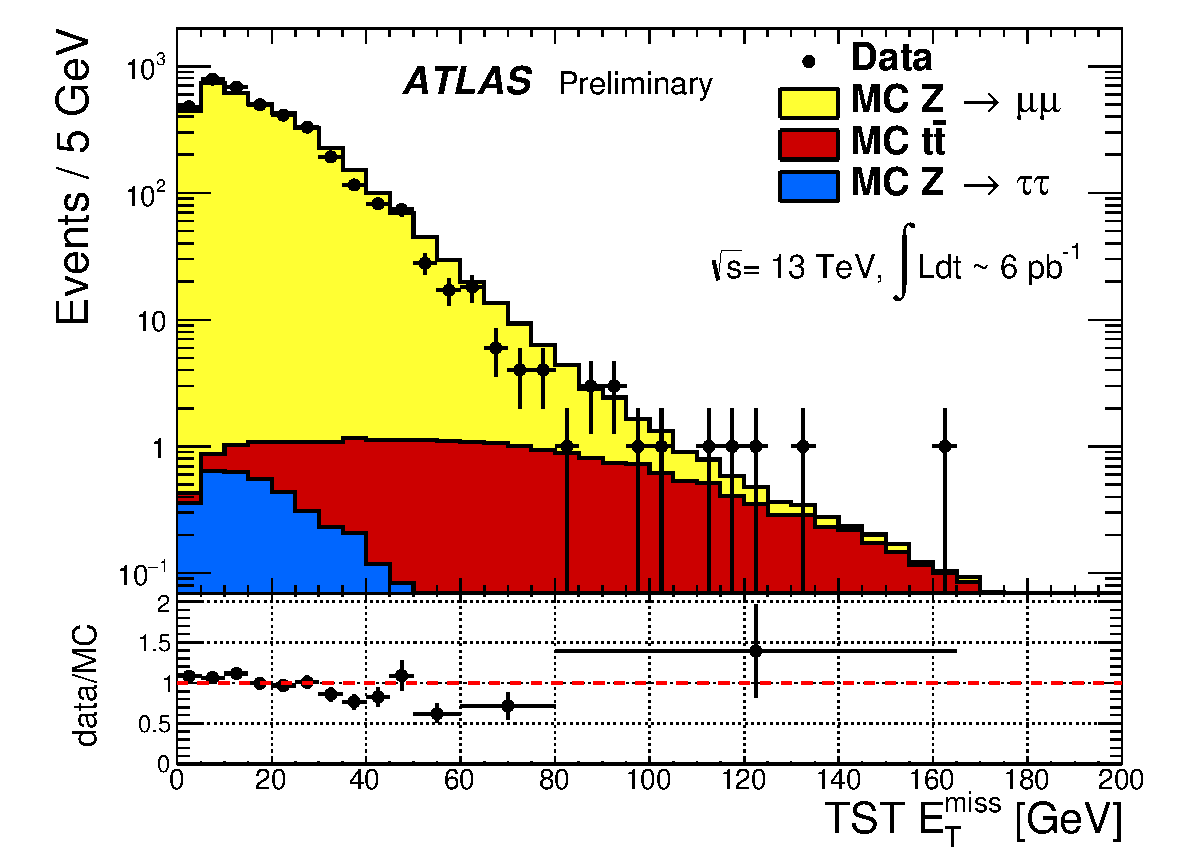
\includegraphics[width=0.95\textwidth]{met_dist}
\subcaption{}
\label{fig:exp.reco.met_dist}
\end{subfigure}
\begin{subfigure}[t]{0.48\textwidth}
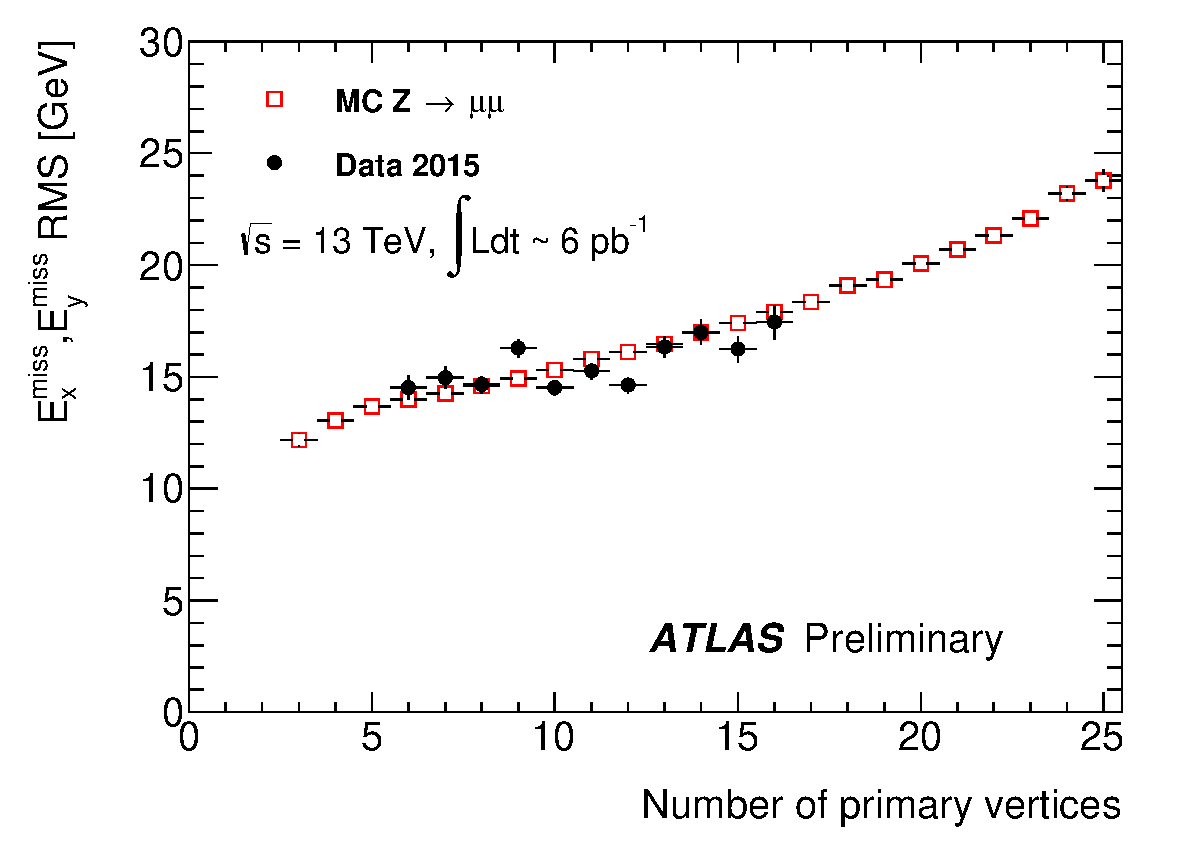
\includegraphics[width=0.95\textwidth]{met_res}
\subcaption{}
\label{fig:exp.reco.met_res}
\end{subfigure}
\vspace{-0.25cm}
\caption{
(a) \met distribution as measured in data with $Z\to\mu\mu$ events without pile-up suppression.
(b) \met resolution as a function of the number of primary vertices in $Z\to\mu\mu$ events. The data (black circles) and MC simulation (red squares) are overlaid. 
}
\label{fig:exp.reco.met}
\end{figure} 
